\documentclass[tikz]{standalone}
\usepackage{pgfplots}
\pgfplotsset{compat=1.18}
\begin{document}
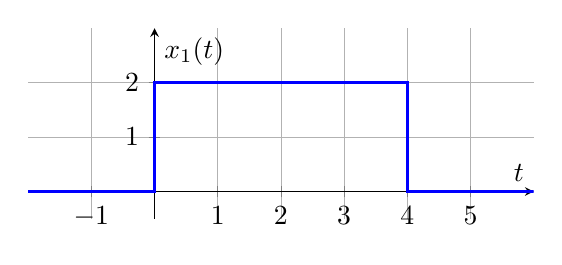
\begin{tikzpicture}
	\begin{axis}[
		width=8cm, height=4cm,
		axis lines=middle,
		xmin=-2, xmax=6, ymin=-0.5, ymax=3,
		xlabel={$t$}, ylabel={$x_1(t)$},
		grid=both,
		grid style={line width=.1pt, draw=gray!40},
		major grid style={line width=.2pt,draw=gray!60},
		xtick={-1,0,1,2,3,4,5}, ytick={0,1,2},
		samples=100
	]
	\addplot[line width=1.2pt, blue] coordinates {(-2,0) (0,0) (0,2) (4,2) (4,0) (6,0)};
	\end{axis}
\end{tikzpicture}
\end{document}
